%%==================================================================%%
%% Author : Abascal Fern�ndez, Patricia                             %%
%% Author : S�nchez Barreiro, Pablo                                 %%
%% Version: 1.2, 15/05/2013                                         %%
%%                                                                  %%
%% Memoria del Proyecto Fin de Carrera                              %%
%% Application Engineering/Generadores de C�digo C#                 %%
%%==================================================================%%

Esta secci�n detalla la secuenciaci�n de las plantillas de generaci�n de c�digo creadas para implementar el algoritmo de la secci�n anterior. La Figura~\ref{app:fig:templates} muestra dicha secuenciaci�n.

\begin{figure}[!tb]
  \center
  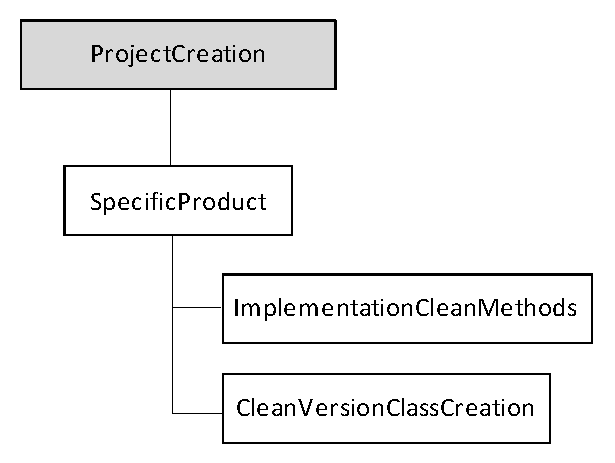
\includegraphics[width=0.35\linewidth]{applicationEngineering/images/TemplatesAppEngineering.eps} \\
  \caption{Secuencia de ejecuci�n de las plantillas de generaci�n de c�digo (Ingenier�a de Aplicaciones)}
  \label{app:fig:templates}
\end{figure}

El punto de partida es id�ntico al utilizado para la fase de \emph{Ingenier�a del Dominio}; es decir, el generador de c�digo llamado \imp{ProjectCreation}, el cual crea el proyecto \emph{Visual Studio 2010} para el producto concreto. Este plantilla invoca a su vez a la plantilla \imp{SpecificProduct}, que es la que gobierna el proceso de generaci�n de c�digo a nivel de \emph{Ingenier�a de la Aplicaci�n}. Para ello, se invocan las dos siguientes plantillas principales.

La plantilla \imp{CalculateClassesAndCleanMethods} recorre todos los caminos existentes en el modelo de la arquitectura concreta, desde el paquete hoja a la ra�z, calculando las clases que hay que crear, las versiones limpias de m�todos a generar, as� como las versiones sucias en las cuales delegar, teniendo en cuenta los conceptos de independencia y alcanzabilidad.
A continuaci�n, se invoca la plantilla \imp{CleanVersionClassGeneration} para cada una de las clases calculadas anteriormente. Para cada clase calculada, se procede a generar todo el c�digo fuente necesario. Resaltar que estas clases, a diferencia de las generadas a nivel de \emph{Ingenier�a del Dominio}, s� son completamente ejecutables y contienen todo el c�digo necesario para ejecutar el producto completo.

Cada una de estas plantillas hace uso a su vez de otras subplantillas, que al igual que en la fase de \emph{Ingenier�a del Dominio}, se han obviado por razones de espacio y claridad.

Una vez implementados los generadores de c�digo para la fase de \emph{Ingenier�a de Aplicaci�n}, procedimos a realizar las pruebas pertinentes.
